TODO.




\subsection{Our Contributions}

This report introduces GVE-Leiden\footnote{https://github.com/puzzlef/leiden-communities-openmp}, an optimized parallel implementation of the Leiden algorithm for community detection on shared memory multicores. On a machine with two 16-core Intel Xeon Gold 6226R processors, GVE-Leiden achieves a processing rate of $352 M$ edges/s on a $3.8 B$ edge graph, and outperforms the original Leiden implementation, igraph Leiden, and NetworKit Leiden by $373\times$, $86\times$, and $7.2\times$ respectively, while identifying communities of the same quality as the first two implementations, and $26\%$ higher quality than NetworKit. Compared to GVE-Louvain, our parallel Louvain implementation, GVE-Leiden achieves an $11$-fold reduction in internally-disconnected communities, with only a $36\%$ increase in computation time. With doubling of threads, GVE-Leiden exhibits an average performance scaling of $1.6\times$.\ignore{This makes GVE-Leiden an attractive choice for high-quality community detection on massive graphs.}




%% - Use --- for a dash.
%% - Use ``camera-ready'' for quotes.
%% - Use {\itshape very} or \textit{very} for italicized text.
%% - Use \verb|acmart| or {\verb|acmart|} for mono-spaced text.
%% - Use \url{https://capitalizemytitle.com/} for URLs.
%% - Use {\bfseries Do not modify this document.} for important boldface details.
%% - Use \ref{fig:name} for referencing.

%% For a block of pre-formatted text: 
% \begin{verbatim}
%   \renewcommand{\shortauthors}{McCartney, et al.}
% \end{verbatim}

%% For a list of items:
% \begin{itemize}
% \item the ``ACM Reference Format'' text on the first page.
% \item the ``rights management'' text on the first page.
% \item the conference information in the page header(s).
% \end{itemize}

%% For a table:
% \begin{table}
%   \caption{Frequency of Special Characters}
%   \label{tab:freq}
%   \begin{tabular}{ccl}
%     \toprule
%     Non-English or Math&Frequency&Comments\\
%     \midrule
%     \O & 1 in 1,000& For Swedish names\\
%     $\pi$ & 1 in 5& Common in math\\
%     \$ & 4 in 5 & Used in business\\
%     $\Psi^2_1$ & 1 in 40,000& Unexplained usage\\
%   \bottomrule
% \end{tabular}
% \end{table}

%% For a full-width table:
% \begin{table*}
%   \caption{Some Typical Commands}
%   \label{tab:commands}
%   \begin{tabular}{ccl}
%     \toprule
%     Command &A Number & Comments\\
%     \midrule
%     \texttt{{\char'134}author} & 100& Author \\
%     \texttt{{\char'134}table}& 300 & For tables\\
%     \texttt{{\char'134}table*}& 400& For wider tables\\
%     \bottomrule
%   \end{tabular}
% \end{table*}


%% For inline math:
% \begin{math}
%   \lim_{n\rightarrow \infty}x=0
% \end{math},

%% For a numbered equation:
% \begin{equation}
%   \lim_{n\rightarrow \infty}x=0
% \end{equation}

%% For an unnumbered equation:
% \begin{displaymath}
%   \sum_{i=0}^{\infty} x + 1
% \end{displaymath}

%% For a figure:
% \begin{figure}[h]
%   \centering
%   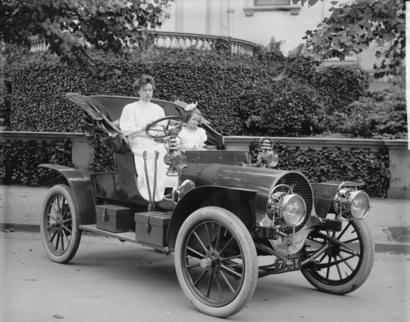
\includegraphics[width=\linewidth]{inc/sample-franklin}
%   \caption{1907 Franklin Model D roadster. Photograph by Harris \&
%     Ewing, Inc. [Public domain], via Wikimedia
%     Commons. (\url{https://goo.gl/VLCRBB}).}
%   \Description{A woman and a girl in white dresses sit in an open car.}
% \end{figure}

%% For a teaser figure.
% \begin{teaserfigure}
%   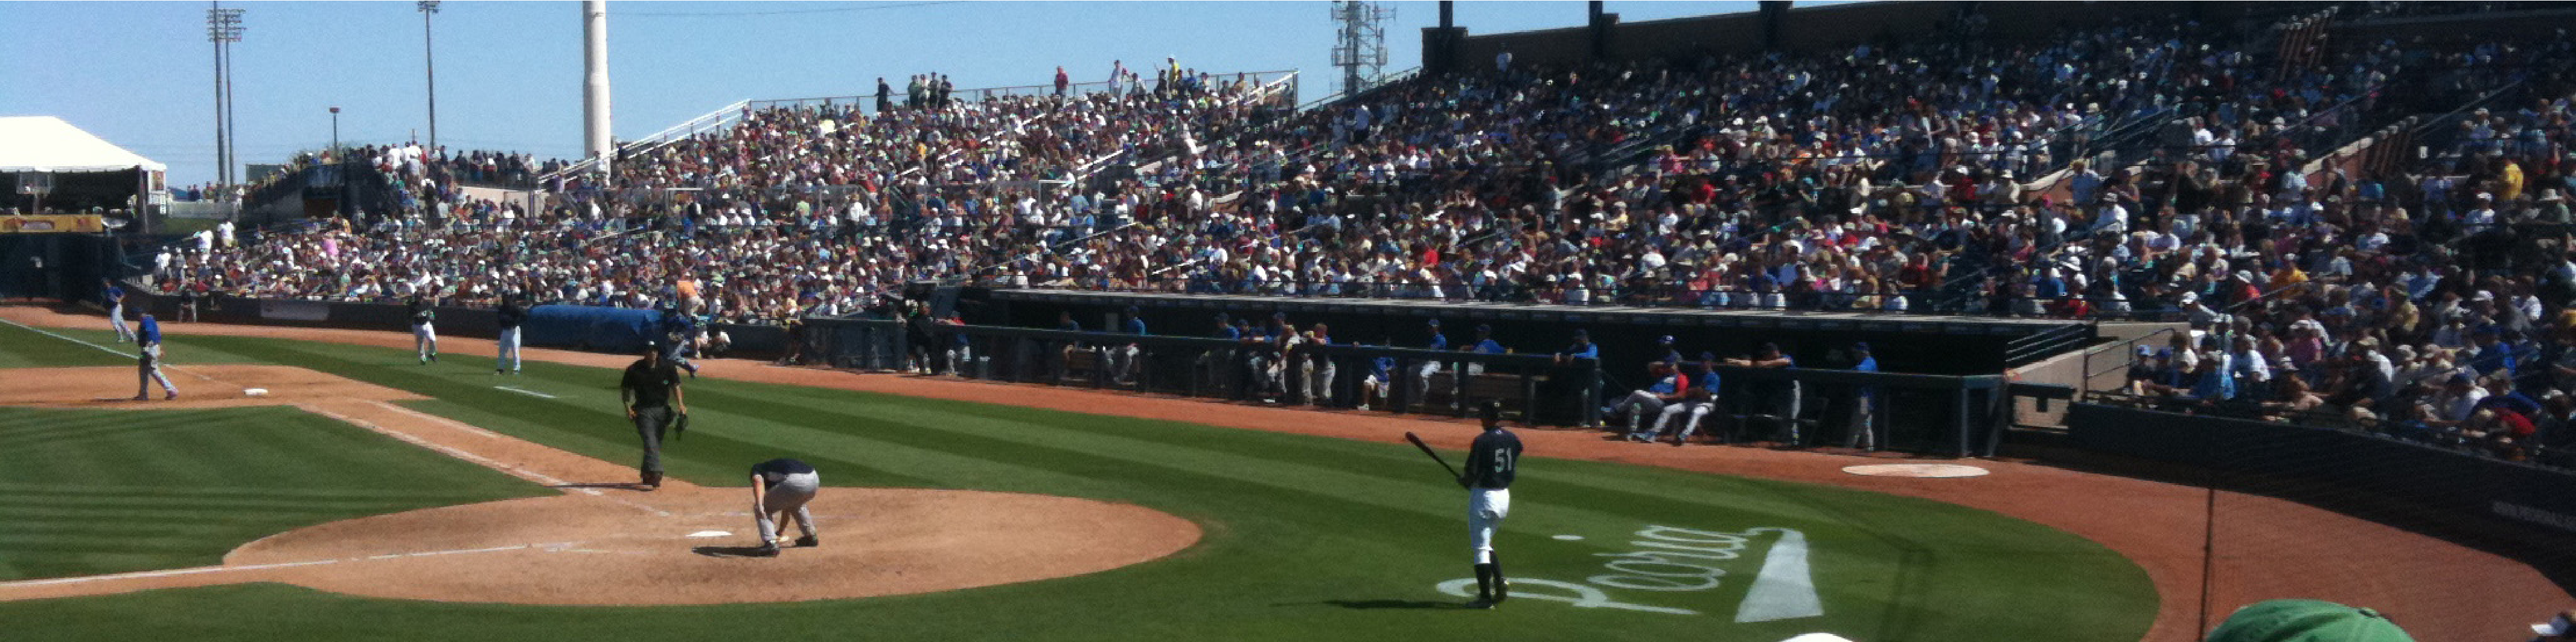
\includegraphics[width=\textwidth]{sampleteaser}
%   \caption{figure caption}
%   \Description{figure description}
% \end{teaserfigure}
